\documentclass[12pt]{book}

% === PACKAGES ===
\usepackage{amsmath, amssymb, amsthm}
\usepackage{multicol, enumitem, xcolor, lipsum, graphicx, hyperref}
\usepackage[margin=1in]{geometry}
\usepackage{tikz}
\usepackage{pgffor}
\usepackage{fancyhdr}
\usepackage{listings}
\usepackage{catchfile}
\usepackage{titlesec}

% === PAGE STYLE ===
\pagestyle{fancy}
\fancyhf{}
\fancyhead[L]{CS2: Object-Oriented Programming}
\fancyhead[R]{\leftmark}
\fancyfoot[C]{\thepage}

% === CODE LISTINGS STYLE ===
\lstset{
  basicstyle=\ttfamily\small,
  backgroundcolor=\color{gray!5},
  frame=single,
  rulecolor=\color{gray!40},
  breaklines=true,
  postbreak=\mbox{\textcolor{gray}{$\hookrightarrow$}\space},
  showstringspaces=false,
  keywordstyle=\color{blue!70!black}\bfseries,
  commentstyle=\color{gray!60}\itshape,
  stringstyle=\color{teal!70!black},
  captionpos=b
}

% === SECTION FORMATTING ===
\titleformat{\chapter}[display]
  {\bfseries\Large}
  {\filright\Huge\thechapter}
  {1ex}
  {\titlerule\vspace{1ex}\filright}
  [\vspace{1ex}\titlerule]

\titleformat{\section}
  {\bfseries\large}
  {\thesection}{1em}{}

% === TITLE INFO ===
\title{CS2 Workbook: Object-Oriented Programming (Chapter 9)}
\author{Jeremy Evert \\ Southwestern Oklahoma State University}
\date{\today}

\begin{document}

% === FRONT MATTER ===
\maketitle
\tableofcontents
\newpage

% === CHAPTERS ===
% Add or remove chapters as you develop them.

% === AUTOLOAD CHAPTERS ===
\chapter{Classes: Introduction}

\section{Grouping Related Items into Objects}

The physical world is made up of materials such as \textbf{wood}, \textbf{metal}, \textbf{plastic}, and \textbf{fabric}.
To make sense of it, we group materials into higher-level concepts such as \textit{chairs}, \textit{tables}, and \textit{televisions}.
Similarly, in programming, we group lower-level data and functions into \textbf{objects}.

\begin{quote}
An \textbf{object} is a bundle of data (variables) and the operations (methods) that act on that data.
\end{quote}

\subsection*{Example: Thinking in Objects}

\begin{center}
\begin{tabular}{|l|l|}
\hline
\textbf{Object} & \textbf{Operations (Methods)} \\
\hline
Chair & \texttt{sit()} \\
Couch & \texttt{sit()}, \texttt{lie\_down()} \\
Drawer & \texttt{put\_item()}, \texttt{take\_item()} \\
\hline
\end{tabular}
\end{center}

Objects let us think about the world in terms of \emph{what things do}, rather than what they are made of.

\subsection*{Participation Discussion}
\begin{itemize}
  \item What real-world object do you interact with daily that could be modeled as a class?
  \item What are its attributes (data) and behaviors (methods)?
\end{itemize}

\subsection{Programs Viewed as Objects}

A program consists of variables and functions, but object-oriented programming encourages us to group related data and actions together.

\begin{center}
\begin{tabular}{|l|l|}
\hline
\textbf{Object Type} & \textbf{Possible Actions} \\
\hline
Restaurant & \texttt{set\_name()}, \texttt{add\_cuisine()}, \texttt{add\_review()} \\
Hotel & \texttt{set\_name()}, \texttt{add\_amenity()}, \texttt{add\_review()} \\
\hline
\end{tabular}
\end{center}

\noindent
\textit{By organizing code this way, we create programs that are easier to read, extend, and maintain.}

\section{Abstraction and Information Hiding}

Abstraction occurs when we use an interface (like an oven’s knob) to hide complex inner details (like heating elements).

\begin{quote}
Objects simplify complexity by hiding details and exposing only essential operations.
\end{quote}

\textbf{Example:}
\begin{center}
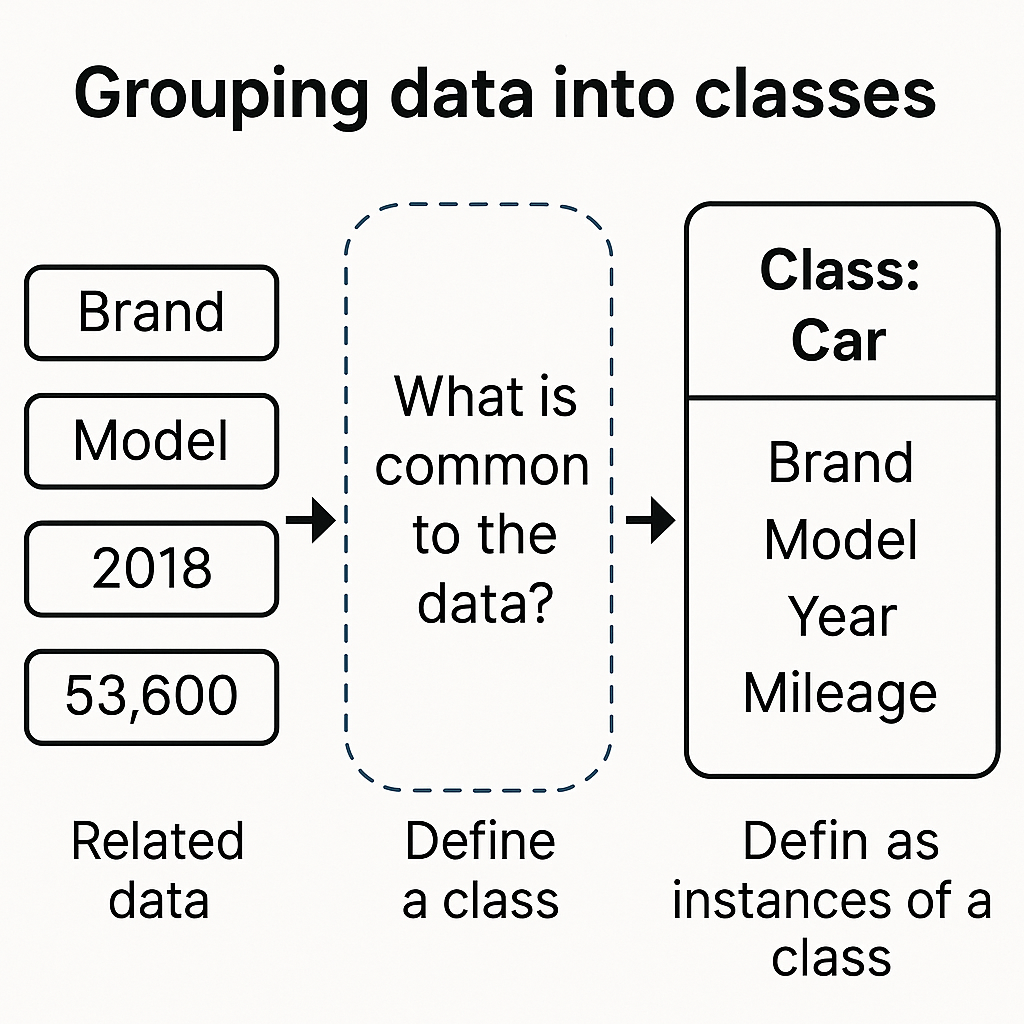
\includegraphics[width=0.8\textwidth]{../images/oven_abstraction_example.png}
\end{center}

\begin{itemize}
  \item A car hides the details of its engine behind a steering wheel, pedals, and a dashboard.
  \item A Python object hides the details of its data, offering you methods like \texttt{.append()} or \texttt{.lower()}.
\end{itemize}

\section{Built-in Objects in Python}

Python automatically provides built-in objects, like:
\begin{itemize}
  \item \texttt{str} — string data type (ex: \texttt{"Hello"})
  \item \texttt{int} — integer data type (ex: \texttt{42})
\end{itemize}

\textbf{Example:}
\begin{verbatim}
s1 = "Hello!"
print(s1.upper())   # Output: HELLO!
i1 = 130
print(i1.bit_length())  # Output: 8
\end{verbatim}

\textit{Even built-in types are objects with data and methods!}

\section*{Reflection Questions}

\begin{enumerate}
  \item What does it mean to say “a program is made of objects”?
  \item Why does abstraction make code easier to understand?
  \item Can you think of three real-world items that could become classes in code?
\end{enumerate}


\chapter{Classes: Grouping Data}

\section{Why Group Data into Classes?}

Many variables in a program are closely related and should be bundled together.
For instance, a time value consists of hours and minutes.
Instead of managing two separate variables, we can define a \textbf{class} that groups them into one logical unit.

\begin{quote}
A \textbf{class} defines a new data type that groups related data (called \emph{attributes}) and the operations that act on them (called \emph{methods}).
\end{quote}

\section{Constructing a Simple Class}

\subsection*{The \texttt{class} Keyword}

\begin{verbatim}
class ClassName:
    # Statement-1
    # Statement-2
    # ...
    # Statement-N
\end{verbatim}

A class defines both the data and the behaviors of an object.
The example below defines a class named \texttt{Time} with two attributes.

\subsection*{Example: Defining a Class with Two Data Attributes}

\begin{verbatim}
class Time:
    """A class that represents a time of day."""
    def __init__(self):
        self.hours = 0
        self.minutes = 0
\end{verbatim}

Here, the \texttt{\_\_init\_\_()} function is a special method called a \textbf{constructor}.
It runs automatically when a new object (or instance) of \texttt{Time} is created.

\section{Creating and Using an Object}

\begin{verbatim}
my_time = Time()
my_time.hours = 7
my_time.minutes = 15

print(f"{my_time.hours} hours and {my_time.minutes} minutes")
\end{verbatim}

\textbf{Output:}
\begin{verbatim}
7 hours and 15 minutes
\end{verbatim}

Each variable created from the class (\texttt{my\_time}) is called an \textbf{instance}.
The attributes of that instance are accessed using the \textbf{dot operator} (\texttt{.}).

\section{Multiple Instances of a Class}

You can create multiple independent instances, each maintaining its own data.

\begin{verbatim}
time1 = Time()
time1.hours = 7
time1.minutes = 30

time2 = Time()
time2.hours = 12
time2.minutes = 45

print(f"{time1.hours} hours and {time1.minutes} minutes")
print(f"{time2.hours} hours and {time2.minutes} minutes")
\end{verbatim}

\textbf{Output:}
\begin{verbatim}
7 hours and 30 minutes
12 hours and 45 minutes
\end{verbatim}

\section{Key Terms}

\begin{description}
    \item[class] A grouping of related data and behaviors.
    \item[attribute] A variable stored within a class or instance.
    \item[method] A function that belongs to a class.
    \item[\_\_init\_\_] The constructor method called automatically when creating a new object.
    \item[self] Refers to the instance itself within class methods.
    \item[instance] An individual object created from a class.
\end{description}

\section{Practice Activity}

\subsection*{Activity 9.2.1 – Define and Instantiate a Class}

\begin{verbatim}
class Person:
    def __init__(self):
        self.name = ""

person1 = Person()
person1.name = "Van"
print(f"This is {person1.name}")
\end{verbatim}

\textbf{Output:}
\begin{verbatim}
This is Van
\end{verbatim}

\subsection*{Activity 9.2.2 – Create Your Own Class}

Define a class called \texttt{BookData} with three attributes:
\texttt{year\_published}, \texttt{title}, and \texttt{num\_chapters}.
Create an instance of the class and assign values to its attributes.

\begin{verbatim}
class BookData:
    def __init__(self):
        self.year_published = 0
        self.title = "Unknown"
        self.num_chapters = 0

my_book = BookData()
my_book.year_published = 2001
my_book.title = "A Tale of Two Cities"
my_book.num_chapters = 45

print(f"{my_book.title} ({my_book.year_published}) has {my_book.num_chapters} chapters.")
\end{verbatim}

\textbf{Output:}
\begin{verbatim}
A Tale of Two Cities (2001) has 45 chapters.
\end{verbatim}

\section*{Reflection Questions}
\begin{enumerate}
    \item What is the difference between a class and an instance?
    \item Why is the \texttt{self} keyword required in class definitions?
    \item How does \texttt{\_\_init\_\_()} help organize data?
\end{enumerate}


\chapter{Instance Methods}

\section{What Are Instance Methods?}

A \textbf{method} is a function that belongs to a class.  
An \textbf{instance method} operates on a specific object created from that class.

Each method must include the special first parameter \texttt{self}, which refers to the current instance of the class.

\section{Example: Adding a Method to a Class}

\begin{verbatim}
class Time:
    def __init__(self):
        self.hours = 0
        self.minutes = 0

    def print_time(self):
        print(f"Hours: {self.hours}", end=" ")
        print(f"Minutes: {self.minutes}")

time1 = Time()
time1.hours = 7
time1.minutes = 15
time1.print_time()
\end{verbatim}

\textbf{Output:}
\begin{verbatim}
Hours: 7 Minutes: 15
\end{verbatim}

---

\section{Understanding \texttt{self}}

The first parameter \texttt{self} provides a reference to the instance itself.  
When a method is called using dot notation, like \texttt{time1.print\_time()},  
Python automatically passes the instance (\texttt{time1}) as the first argument.

---

\section{Adding Behavior to a Class}

You can add more methods to model real behavior.  
The example below shows an \texttt{Employee} class with a method that calculates pay.

\begin{verbatim}
class Employee:
    def __init__(self):
        self.wage = 0
        self.hours_worked = 0

    def calculate_pay(self):
        return self.wage * self.hours_worked

alice = Employee()
alice.wage = 9.25
alice.hours_worked = 35
print(f"Alice's Net Pay: ${alice.calculate_pay():.2f}")
\end{verbatim}

\textbf{Output:}
\begin{verbatim}
Alice's Net Pay: $323.75
\end{verbatim}

---

\section{Common Mistake: Forgetting \texttt{self}}

If you forget to include \texttt{self} as the first parameter of a method, Python will raise an error:

\begin{verbatim}
class Employee:
    def __init__(self):
        self.wage = 0
        self.hours_worked = 0

    def calculate_pay():
        return self.wage * self.hours_worked

alice = Employee()
alice.wage = 9.25
alice.hours_worked = 35
print(alice.calculate_pay())
\end{verbatim}

\textbf{Error:}
\begin{verbatim}
TypeError: calculate_pay() takes 0 positional arguments but 1 was given
\end{verbatim}

---

\section{Practice: Define and Use a Method}

\textbf{Example Activity 9.3.1 – Adding a Method}

\begin{verbatim}
class Person:
    def __init__(self):
        self.first_name = ""

    def print_name(self):
        print(f"He is {self.first_name}")

person1 = Person()
person1.first_name = "Bob"
person1.print_name()
\end{verbatim}

\textbf{Output:}
\begin{verbatim}
He is Bob
\end{verbatim}

---

\section{Challenge: Seat Class with Instance Method}

\begin{verbatim}
class Seat:
    def __init__(self):
        self.row = 0
        self.col = 0

    def print_attributes(self):
        print(f"Row: {self.row}, Column: {self.col}")

seat1 = Seat()
seat1.row = 3
seat1.col = 5
seat1.print_attributes()
\end{verbatim}

\textbf{Output:}
\begin{verbatim}
Row: 3, Column: 5
\end{verbatim}


\chapter{Class and Instance Object Types}

\section*{9.4.1 Understanding Class vs. Instance Objects}

A class in Python acts as a \textbf{factory} that creates \textbf{instance objects}. 
Each instance has its own data (attributes), but shares the same methods defined in the class.

\begin{verbatim}
class Time:
    def __init__(self):
        self.hours = 0
        self.minutes = 0

time1 = Time()
time2 = Time()
time1.hours = 5
time2.hours = 7
\end{verbatim}

---

\section*{9.4.2 Class Attributes vs. Instance Attributes}

A \textbf{class attribute} is shared by all instances, while an \textbf{instance attribute} is unique to each object.

\begin{verbatim}
class MarathonRunner:
    race_distance = 42.195  # Class attribute

    def __init__(self):
        self.speed = 0      # Instance attribute

runner1 = MarathonRunner()
runner2 = MarathonRunner()
runner1.speed = 7.5
runner2.speed = 3.0
print(f"Runner1: {runner1.speed}, Runner2: {runner2.speed}")
\end{verbatim}


---

\section*{9.4.3 Key Concept Summary}

\begin{itemize}
    \item \textbf{Class Object:} A template that defines data and behavior.
    \item \textbf{Instance Object:} A unique copy created from the class.
    \item \textbf{Class Attribute:} Shared by all instances.
    \item \textbf{Instance Attribute:} Belongs only to one instance.
\end{itemize}

---

\section*{9.4.4 Practice Activity}

Modify the code below to add a method \texttt{print\_attributes()} 
that prints both the class attribute and the instance attribute values.

\begin{verbatim}
class PhoneNumber:
    area_code = "405"

    def __init__(self):
        self.number = "555-1234"

# TODO: Add print_attributes method
\end{verbatim}

\begin{center}
\textit{What happens if you change the class attribute after creating multiple instances?}
\end{center}


\chapter{Class Example: Seat Reservation System}

\section*{9.5 Class Example – Airline Seat Reservation System}

A \textbf{class} can represent a real-world entity that manages its own data and actions.  
The example below models a simple airline seat reservation system. Each \texttt{Seat} object stores a passenger’s name and the amount paid.

\begin{verbatim}
class Seat:
    def __init__(self):
        self.first_name = ""
        self.last_name = ""
        self.paid = 0.0

    def reserve(self, f_name, l_name, amt_paid):
        self.first_name = f_name
        self.last_name = l_name
        self.paid = amt_paid

    def make_empty(self):
        self.first_name = ""
        self.last_name = ""
        self.paid = 0.0

    def is_empty(self):
        return self.first_name == ""

    def print_seat(self):
        print(f"{self.first_name} {self.last_name}, Paid: {self.paid:.2f}")


def make_seats_empty(seats):
    for s in seats:
        s.make_empty()


def print_seats(seats):
    for i in range(len(seats)):
        print(f"{i}:", end=" ")
        seats[i].print_seat()


num_seats = 5
available_seats = []

for i in range(num_seats):
    available_seats.append(Seat())

command = input("Enter command (p/r/q):\n")

while command != "q":
    if command == "p":  # Print seats
        print_seats(available_seats)
    elif command == "r":  # Reserve a seat
        seat_num = int(input("Enter seat num:\n"))
        if not available_seats[seat_num].is_empty():
            print("Seat not empty")
        else:
            fname = input("Enter first name:\n")
            lname = input("Enter last name:\n")
            paid = float(input("Enter amount paid:\n"))
            available_seats[seat_num].reserve(fname, lname, paid)
    else:
        print("Invalid command.")

    command = input("Enter command (p/r/q):\n")
\end{verbatim}

\subsection*{Discussion}
This example demonstrates:
\begin{itemize}
    \item Encapsulation of related data and behaviors within a class.
    \item The use of methods to modify and access object state.
    \item A program structure that makes expansion (like saving or loading seats) simple.
\end{itemize}



\chapter{Class Constructors}
\label{ch:class_constructors}

\section*{9.6 Overview}
A class constructor is a special method that defines how new objects are created and initialized.
In Python, the constructor method is named \texttt{\_\_init\_\_()}.
Constructors are used to set up instance attributes and can accept parameters to configure each new object.

---

\section*{Adding Parameters to a Constructor}

\begin{lstlisting}[language=Python, caption={A simple constructor with parameters.}]
class RaceTime:
    def __init__(self, start_time, end_time, distance):
        """Initialize race data."""
        self.start_time = start_time    # Format: "H:MM"
        self.end_time = end_time
        self.distance = distance        # In miles

# Create RaceTime objects
time_jason = RaceTime("3:15", "7:45", 26.21875)
time_bobby = RaceTime("3:15", "6:30", 26.21875)
\end{lstlisting}

Here, each new object receives its starting time, ending time, and race distance.
This is more powerful than setting everything to zero — each instance can have its own data immediately upon creation.

---

\section*{Complete RaceTime Example}

\begin{lstlisting}[language=Python, caption={RaceTime class with methods.}]
class RaceTime:
    def __init__(self, start_hrs, start_mins, end_hrs, end_mins, dist):
        self.start_hrs = start_hrs
        self.start_mins = start_mins
        self.end_hrs = end_hrs
        self.end_mins = end_mins
        self.distance = dist

    def print_time(self):
        if self.end_mins >= self.start_mins:
            minutes = self.end_mins - self.start_mins
            hours = self.end_hrs - self.start_hrs
        else:
            minutes = 60 - self.start_mins + self.end_mins
            hours = self.end_hrs - self.start_hrs - 1
        print(f"Time to complete race: {hours}:{minutes:02d}")

    def print_pace(self):
        total_minutes = (self.end_hrs * 60 + self.end_mins) - \
                        (self.start_hrs * 60 + self.start_mins)
        pace = total_minutes / self.distance
        print(f"Average pace: {pace:.2f} mins/mile")

# Example interaction
distance = 5.0
start_hrs = int(input("Enter starting time hours: "))
start_mins = int(input("Enter starting time minutes: "))
end_hrs = int(input("Enter ending time hours: "))
end_mins = int(input("Enter ending time minutes: "))

race_time = RaceTime(start_hrs, start_mins, end_hrs, end_mins, distance)
race_time.print_time()
race_time.print_pace()
\end{lstlisting}

---

\section*{Default Constructor Parameters}

Constructors can also include default values for convenience.  
This reduces repetition and helps when typical defaults are common.

\begin{lstlisting}[language=Python, caption={Employee class with default parameters.}]
class Employee:
    def __init__(self, name, wage=8.25, hours=20):
        """Default employee works part-time and earns minimum wage."""
        self.name = name
        self.wage = wage
        self.hours = hours

employees = [
    Employee("Todd"),                   # uses defaults
    Employee("Jason"),                  # uses defaults
    Employee("Tricia", 12.50, 40)       # manager: custom values
]

for e in employees:
    print(f"{e.name} earns ${e.wage * e.hours:.2f} per week")
\end{lstlisting}

---

\section*{Constructors in Practice: Student Example}

\begin{lstlisting}[language=Python, caption={Constructor with several defaults.}]
class Student:
    def __init__(self, name, grade=9, honors=False, athletics=False):
        self.name = name
        self.grade = grade
        self.honors = honors
        self.athletics = athletics

johnny = Student("Johnny", grade=11, honors=True)
tommy = Student("Tommy")

print(f"{johnny.name}: grade {johnny.grade}, honors={johnny.honors}")
print(f"{tommy.name}: grade {tommy.grade}, athletics={tommy.athletics}")
\end{lstlisting}

---

\section*{Constructor Exercises}

\begin{enumerate}
    \item Modify \texttt{Employee} so that it tracks yearly pay in addition to hourly.
    \item Add a method \texttt{is\_manager()} that returns \texttt{True} if wage > 12.
    \item Rewrite \texttt{RaceTime} so that it accepts total minutes instead of hours and minutes separately.
\end{enumerate}


\chapter{Class Interfaces}
\label{ch:09_07_class_interfaces}

\section*{Overview}
A \textbf{class interface} defines the set of methods that a programmer uses to interact with an instance of a class.  
The interface describes \emph{what} operations can be performed on an object, while the \textbf{implementation} describes \emph{how} those operations work internally.

In this section, we will explore:
\begin{itemize}
    \item How to design class interfaces for readability and reuse.
    \item How to separate interface from implementation.
    \item The use of internal methods to simplify class logic.
\end{itemize}

\vspace{1em}
\noindent
\textbf{Key Idea:} A well-designed class acts like a mini toolbox---you can use its tools (the methods) without worrying about how each tool is built inside.

\section{Example: The RaceTime Class Interface}

Consider the following example that models a simple race timer.  
The interface includes three methods:
\begin{itemize}
    \item \texttt{\_\_init\_\_()} — creates a new RaceTime instance.
    \item \texttt{print\_time()} — prints the time to complete the race.
    \item \texttt{print\_pace()} — prints the average pace per mile.
\end{itemize}

\begin{lstlisting}[language=Python, caption={A class interface consists of methods to interact with an instance.}]
class RaceTime:
    def __init__(self, start_time, end_time, distance):
        self.start_time = start_time
        self.end_time = end_time
        self.distance = distance

    def print_time(self):
        # Implementation details hidden from user
        ...

    def print_pace(self):
        # Implementation details hidden from user
        ...
\end{lstlisting}

\vspace{1em}
\noindent
\textbf{Instructor Note:} Emphasize that users of the class only need to know how to call \texttt{print\_time()} or \texttt{print\_pace()}, not how they compute their results internally.

\begin{center}
\includegraphics[width=0.8\textwidth]{images/class_interfaces_diagram.png}
\captionof{figure}{Visual overview of a class interface and its hidden implementation.}
\end{center}

\section{Internal (Private) Methods}
Sometimes, a class includes internal helper methods that are not meant to be accessed directly.  
By convention, these methods begin with an underscore (\_), signaling to programmers that they are used only inside the class.

\begin{lstlisting}[language=Python, caption={RaceTime class with internal helper method.}]
class RaceTime:
    def __init__(self, start_hrs, start_mins, end_hrs, end_mins, dist):
        self.start_hrs = start_hrs
        self.start_mins = start_mins
        self.end_hrs = end_hrs
        self.end_mins = end_mins
        self.dist = dist

    def print_time(self):
        total_time = self._diff_time()
        print(f"Time to complete race: {total_time[0]}:{total_time[1]:02}")

    def print_pace(self):
        total_time = self._diff_time()
        total_minutes = total_time[0]*60 + total_time[1]
        print(f"Avg pace (mins/mile): {total_minutes / self.dist:.2f}")

    def _diff_time(self):
        """Internal helper method"""
        if self.end_mins >= self.start_mins:
            minutes = self.end_mins - self.start_mins
            hours = self.end_hrs - self.start_hrs
        else:
            minutes = 60 - self.start_mins + self.end_mins
            hours = self.end_hrs - self.start_hrs - 1
        return (hours, minutes)
\end{lstlisting}

\section{Abstract Data Types (ADTs) and Information Hiding}
A class can also represent an \textbf{Abstract Data Type (ADT)}, which hides the details of how data is stored or manipulated internally.  
The ADT provides a public interface for the user while keeping private methods and variables hidden.

\begin{itemize}
    \item The user sees the interface (the public methods).
    \item The developer maintains control of the internal logic.
    \item This separation prevents accidental misuse and simplifies debugging.
\end{itemize}

\vspace{1em}
\noindent
In Python, private members are not enforced, but the underscore convention signals to other programmers that a method is intended for internal use only.

\begin{quote}
\textit{“An ADT is like a vending machine—you press a button, and magic happens inside.”}
\end{quote}

\section{Quick Review}
\begin{enumerate}
    \item The \textbf{interface} of a class defines what users can do with it.
    \item The \textbf{implementation} defines how it does those things.
    \item Internal methods usually begin with an underscore (\_).
    \item A well-designed class separates its interface from its implementation.
\end{enumerate}

\section*{Participation Check}
\begin{itemize}
    \item True or False: A class interface consists of methods that a programmer should use to modify or access the class.
    \item True or False: Internal methods should begin with an underscore in their name.
    \item True or False: Internal methods cannot be called outside the class.
    \item True or False: A well-designed class separates its interface from its implementation.
\end{itemize}

\vspace{2em}
\noindent
\textbf{Next Up:} In Section 9.8, we’ll learn about \textit{class customization}—defining how objects behave with built-in operators like \texttt{==}, \texttt{<}, or \texttt{+}.


\chapter{Class Customization}

\section*{9.8 Class Customization}

\textbf{Class customization} is the process of defining how an instance of a class should behave
for certain operations—such as printing, comparing, or arithmetic.  
Python provides \textit{special method names} (sometimes called “dunder methods”) that begin
and end with double underscores.  
By defining these, programmers can customize how built-in behaviors interact with objects.

\subsection*{Implementing \_\_str\_\_(): Custom Printing}

\noindent\textbf{Example 9.8.1:} Implementing \_\_str\_\_ alters how the class is printed.

\begin{multicols}{2}
\textbf{Normal Printing:}
\begin{lstlisting}[language=Python]
class Toy:
    def __init__(self, name, price, min_age):
        self.name = name
        self.price = price
        self.min_age = min_age

truck = Toy("Monster Truck XX", 14.99, 5)
print(truck)
\end{lstlisting}

\columnbreak
\textbf{Customized Printing:}
\begin{lstlisting}[language=Python]
class Toy:
    def __init__(self, name, price, min_age):
        self.name = name
        self.price = price
        self.min_age = min_age

    def __str__(self):
        return (f"{self.name} costs only ${self.price:.2f}. "
                f"Not for children under {self.min_age}!")

truck = Toy("Monster Truck XX", 14.99, 5)
print(truck)
\end{lstlisting}
\end{multicols}

\noindent Output:
\begin{verbatim}
Monster Truck XX costs only $14.99. Not for children under 5!
\end{verbatim}

\subsection*{Try It: Customizing Print Output}

\begin{lstlisting}[language=Python]
class Car:
    def __init__(self, make, model, year, miles, price):
        self.make = make
        self.model = model
        self.year = year
        self.miles = miles
        self.price = price

    # FIXME: add __str__() to format output
\end{lstlisting}

\noindent
Desired output example:
\begin{verbatim}
1989 Chevrolet Blazer:
Mileage: 115000
Sticker price: $3250
\end{verbatim}

\subsection*{Operator Overloading}

Python also allows classes to redefine built-in operators such as \texttt{<}, \texttt{>}, \texttt{==}, and
\texttt{+}.  This is done through special methods such as \texttt{\_\_lt\_\_}, \texttt{\_\_gt\_\_},
\texttt{\_\_eq\_\_}, etc.

\textbf{Example 9.8.2: Overloading the < Operator}

\begin{lstlisting}[language=Python]
class Time:
    def __init__(self, hours, minutes):
        self.hours = hours
        self.minutes = minutes

    def __str__(self):
        return f"{self.hours}:{self.minutes:02d}"

    def __lt__(self, other):
        if self.hours < other.hours:
            return True
        elif self.hours == other.hours:
            return self.minutes < other.minutes
        return False
\end{lstlisting}

\noindent
These comparison methods are known as \textbf{rich comparison methods}.
\begin{center}
\begin{tabular}{ll}
\textbf{Method} & \textbf{Operator} \\
\hline
\_\_lt\_\_ & less than (<) \\
\_\_le\_\_ & less than or equal (<=) \\
\_\_gt\_\_ & greater than (>) \\
\_\_ge\_\_ & greater than or equal (>=) \\
\_\_eq\_\_ & equal (==) \\
\_\_ne\_\_ & not equal (!=) \\
\end{tabular}
\end{center}

\subsection*{Practice: Comparing Quarterbacks}

\begin{lstlisting}[language=Python]
class Quarterback:
    def __init__(self, yrds, tds, cmps, atts, ints, wins):
        self.wins = wins
        self.rating = (((8.4 * yrds) + (330 * tds)
                        + (100 * cmps) - (200 * ints)) / atts)

    def __lt__(self, other):
        return (self.rating < other.rating or
                self.wins < other.wins)

    def __gt__(self, other):
        return (self.rating > other.rating and
                self.wins > other.wins)
\end{lstlisting}

\subsection*{Challenge: Used Car Comparison}

\begin{lstlisting}[language=Python]
class UsedCar:
    def __init__(self, price, condition):
        self.price = price
        self.condition = condition  # 0=poor, 5=new

    def __lt__(self, other):
        return self.price < other.price

    def __le__(self, other):
        return self.price <= other.price

    def __gt__(self, other):
        return self.condition > other.condition

    def __ne__(self, other):
        return (self.price != other.price or
                self.condition != other.condition)
\end{lstlisting}

\subsection*{Defining \_\_str\_\_ for Custom Output}

\textbf{Challenge:} Define \_\_str\_\_ for a simple CarRecord class.

\begin{lstlisting}[language=Python]
class CarRecord:
    def __init__(self):
        self.year_made = 0
        self.car_vin = ""

    def __str__(self):
        return f"Year: {self.year_made}, VIN: {self.car_vin}"

my_car = CarRecord()
my_car.year_made = 2009
my_car.car_vin = "ABC321"
print(my_car)
\end{lstlisting}

\noindent Output:
\begin{verbatim}
Year: 2009, VIN: ABC321
\end{verbatim}

\subsection*{Reflection}

\begin{itemize}
\item How does \_\_str\_\_ help make debugging easier?
\item Why might you overload comparison operators for a custom class?
\item What risks exist when customizing too many class behaviors?
\end{itemize}

\noindent\textbf{Summary:}
\begin{itemize}
\item Class customization uses special method names (e.g., \_\_str\_\_, \_\_lt\_\_, \_\_eq\_\_).
\item Enables clean printing, sorting, and comparison of class instances.
\item Encourages readable, intuitive code design.
\end{itemize}


\chapter{More Operator Overloading: Classes as Numeric Types}

\section*{9.9 Classes as Numeric Types}

Numeric operators such as \texttt{+}, \texttt{-}, \texttt{*}, and \texttt{/} can be overloaded using class customization techniques.  
A user-defined class can thus be treated as a numeric object in which instances of that class can be added, subtracted, or otherwise combined.  

Consider the example below, which represents a 24-hour clock.  
The algorithm determines the absolute shortest distance between two given times.  
For instance, the time between 5:00 and 3:30 (same day) is shorter than between 22:30 and 2:40 (across midnight).

\begin{lstlisting}[language=Python, caption={Extending the Time class with an overloaded subtraction operator}]
class Time24:
    def __init__(self, hours, minutes):
        self.hours = hours
        self.minutes = minutes

    def __str__(self):
        return f"{self.hours:02d}:{self.minutes:02d}"

    def __gt__(self, other):
        if self.hours > other.hours:
            return True
        elif self.hours == other.hours and self.minutes > other.minutes:
            return True
        return False

    def __sub__(self, other):
        """Calculate absolute distance between two times."""
        if self > other:
            larger, smaller = self, other
        else:
            larger, smaller = other, self

        hrs = larger.hours - smaller.hours
        mins = larger.minutes - smaller.minutes
        if mins < 0:
            mins += 60
            hrs -= 1
        if hrs > 12:
            hrs = 24 - hrs
        return Time24(hrs, mins)

t1 = Time24(5, 0)
t2 = Time24(3, 30)
print(f"Time difference: {t1 - t2}")   # Time difference: 01:30
\end{lstlisting}

\noindent
The \texttt{\_\_sub\_\_()} method defines how subtraction behaves for two \texttt{Time24} instances.  
If \texttt{t1} and \texttt{t2} are both \texttt{Time24} objects, then the expression \texttt{t1 - t2}  
calls \texttt{t1.\_\_sub\_\_(t2)} and returns another \texttt{Time24} instance.

\subsection*{Using \texttt{isinstance()} for Safer Subtraction}

To handle subtraction of arbitrary types, we can use the built-in \texttt{isinstance()} function.  
This ensures that our class behaves predictably even when mixed with other types.

\begin{lstlisting}[language=Python, caption={The isinstance() check in operator overloading}]
class Time24:
    def __init__(self, hours, minutes):
        self.hours = hours
        self.minutes = minutes

    def __str__(self):
        return f"{self.hours:02d}:{self.minutes:02d}"

    def __sub__(self, other):
        # Handle subtraction by integer minutes
        if isinstance(other, int):
            return Time24(self.hours, self.minutes - other)
        elif isinstance(other, Time24):
            hrs = self.hours - other.hours
            mins = self.minutes - other.minutes
            if mins < 0:
                mins += 60
                hrs -= 1
            if hrs < 0:
                hrs += 24
            return Time24(hrs, mins)
        else:
            raise NotImplementedError(f"Unsupported operand type: {type(other)}")

t1 = Time24(10, 15)
print(t1 - 45)              # Subtract 45 minutes
print(t1 - Time24(8, 30))   # Time difference
\end{lstlisting}

\subsection*{Common Operator Methods}

Python allows overloading of almost every arithmetic operator using special methods:

\begin{center}
\begin{tabular}{ll}
\textbf{Method} & \textbf{Description} \\
\hline
\_\_add\_\_(self, other) & Addition (+) \\
\_\_sub\_\_(self, other) & Subtraction (-) \\
\_\_mul\_\_(self, other) & Multiplication (*) \\
\_\_truediv\_\_(self, other) & Division (/) \\
\_\_floordiv\_\_(self, other) & Floor Division (//) \\
\_\_mod\_\_(self, other) & Modulus (\%) \\
\_\_pow\_\_(self, other) & Exponentiation (**) \\
\_\_abs\_\_(self) & Absolute Value (abs()) \\
\_\_int\_\_(self) & Convert to integer (int()) \\
\_\_float\_\_(self) & Convert to float (float()) \\
\end{tabular}
\end{center}

\subsection*{Participation Example: LooseChange Class}

\begin{lstlisting}[language=Python, caption={A simple numeric class using operator overloading}]
class LooseChange:
    def __init__(self, value):
        self.value = value   # total cents

    def __add__(self, other):
        new_value = self.value + other.value
        return LooseChange(new_value)

    def __float__(self):
        return self.value / 100.0

lc1 = LooseChange(135)
lc2 = LooseChange(115)
print(float(lc1 + lc2))   # 2.50
\end{lstlisting}

\subsection*{Challenge Example: Duration Addition}

\begin{lstlisting}[language=Python, caption={Operator overloading for adding durations}]
class Duration:
    def __init__(self, hours, minutes):
        self.hours = hours
        self.minutes = minutes

    def __add__(self, other):
        total_hours = self.hours + other.hours
        total_minutes = self.minutes + other.minutes
        if total_minutes >= 60:
            total_hours += 1
            total_minutes -= 60
        return Duration(total_hours, total_minutes)

first_trip = Duration(1, 35)
second_trip = Duration(0, 43)
total_trip = first_trip + second_trip
print(total_trip.hours, total_trip.minutes)  # Output: 2 18
\end{lstlisting}

\section*{Instructor Notes}

\begin{itemize}
  \item Emphasize how operator overloading enhances readability and reuse.
  \item Students often forget to return a new instance instead of a raw value.
  \item Discuss when operator overloading improves clarity versus when it hides complexity.
\end{itemize}

\bigskip
\noindent
\textbf{Reflection:}  
Encourage students to design a class (e.g., \texttt{BankAccount}, \texttt{Vector2D}, or \texttt{Temperature})  
that uses at least two overloaded operators and one type conversion (\texttt{\_\_float\_\_} or \texttt{\_\_int\_\_}).



\chapter{Memory Allocation and Garbage Collection}
\label{ch:memory_allocation_and_garbage_collection}

\section*{9.10 Memory Allocation and Garbage Collection}

\subsection*{Memory Allocation}

The process of an application requesting and being granted memory is called
\textbf{memory allocation}.  
When a Python program runs, it requests memory from the operating system.
Python’s runtime then divides that memory into sections for code, data, and dynamically
created objects.

While some languages require programmers to manage memory manually,
Python automatically allocates and releases memory on the programmer’s behalf.

\begin{lstlisting}[language=Python, caption={Memory allocation in Python}]
lst = []
for i in range(0, 100):
    lst.append(i)
print("List length:", len(lst))
\end{lstlisting}

When the list \texttt{lst} is created, Python requests space for it from the operating
system. As more elements are appended, the interpreter automatically allocates additional
blocks of memory as needed.

\textbf{Key Points}
\begin{itemize}
  \item System memory is divided into segments managed by the OS.
  \item Python applications request memory through the interpreter, not directly.
  \item Other processes may occupy different regions of memory simultaneously.
  \item Allocation is usually invisible to the programmer.
\end{itemize}

\begin{quote}
\textbf{Instructor Note:} Emphasize that memory allocation happens behind the scenes.
The programmer writes code that creates objects—Python handles where and how they live.
\end{quote}

\subsection*{Quick Check}

\begin{enumerate}
  \item The Python runtime requests memory from the operating system. \textbf{(True)}
  \item Objects may reside in memory that has not been allocated. \textbf{(False)}
  \item All programming languages perform memory allocation for the programmer. \textbf{(False)}
\end{enumerate}

---

\subsection*{Garbage Collection}

\textbf{Memory deallocation} is the act of freeing memory that stores variables or objects
that are no longer needed.  
Python uses a managed model: when objects are no longer referenced by any variable, they
become candidates for automatic removal by the \textbf{garbage collector}.

Each object in memory maintains a \textbf{reference count} (RC)---the number of variables
that reference it. When an object's RC becomes~0, Python knows it can reclaim that space.

\begin{lstlisting}[language=Python, caption={Reference counting in Python}]
string1 = "Python"
string2 = "Computer science"
string3 = string2
string1 = "ZyBooks"
string2 = string1
\end{lstlisting}

Explanation:
\begin{itemize}
  \item Initially, \texttt{string1} references ``Python''.
  \item \texttt{string2} and \texttt{string3} reference ``Computer science''.
  \item Reassigning \texttt{string1} to ``ZyBooks'' makes ``Python'' unreachable.
        Its reference count drops to~0 and it can be deallocated.
\end{itemize}

\begin{quote}
\textbf{Instructor Note:} Demonstrate using a small live example or a diagram to show how
reference counts change as variables are reassigned.
\end{quote}

\textbf{True/False Practice}
\begin{enumerate}
  \item An object with RC~=~0 can be deallocated by the garbage collector. \textbf{True}
  \item Deallocation happens immediately when RC drops to~0. \textbf{False}
  \item Swapping two variables may briefly create an object with RC~=~0. \textbf{True}
\end{enumerate}

---

\subsection*{Reflection}

\begin{itemize}
  \item Why does Python use automatic garbage collection?
  \item How does reference counting prevent memory leaks?
  \item What is one situation where garbage collection might not occur immediately?
\end{itemize}

\begin{quote}
\textbf{Summary:}  
Python automates both allocation and deallocation of memory.
Objects are stored only as long as they are referenced, allowing developers to focus on
logic rather than low-level memory management.
\end{quote}





{
  \input{\chapterfile}
  \clearpage
}

% === END DOCUMENT ===
\end{document}

